%%%%%%%%%%%%%%%%%%%%%%%%%%%%%%%%%%%%%%%%%%%%%%%%%%%
%
%  New template code for TAMU Theses and Dissertations starting Fall 2012.
%  For more info about this template or the
%  TAMU LaTeX User's Group, see http://www.howdy.me/.
%
%  Author: Wendy Lynn Turner
%	 Version 1.0
%  Last updated 8/5/2012
%
%%%%%%%%%%%%%%%%%%%%%%%%%%%%%%%%%%%%%%%%%%%%%%%%%%%

%%%%%%%%%%%%%%%%%%%%%%%%%%%%%%%%%%%%%%%%%%%%%%%%%%%%%%%%%%%%%%%%%%%%%%%
%%%                           Implementation
%%%%%%%%%%%%%%%%%%%%%%%%%%%%%%%%%%%%%%%%%%%%%%%%%%%%%%%%%%%%%%%%%%%%%%

\chapter{\uppercase {Implementation Results}}

\section{Image Synthesis Program Structure and Implementation}

The basis for every ray tracing program can be broken down into a simple set of processes.  First, a program must be able to read and write images.  Once the ability to read and write images has been realized, the process for casting rays can begin. This process is demonstrated by the following pseudocode, or code outline:

\begin{algorithm}[H]
\label{alg:RayTracingPseudocode}
\setstretch{1.0}
 \ForEach{~$pixel$ in ~$image$}{
    \ForEach{$object$ in $scene$}{
        \If{$object$ intersects $ray$}{
               $intersectionDistance$ = distance of viewpoint from intersection of object and ray\;
            \If{$intersection$ \space\textgreater\space $previousIntersection$}{
                $previousIntersection$ = $intersection$\;
                }
                }
    }
    \If{$intersection$ exists}{
        \ForEach{~$Light$ in ~$scene$}{
            determine $materialColor$ from ~$light$\;
        }
        $pixel$ = $materialColor$\;
    }
    \Else{
        $pixel$ = black or alpha(no color)
    }
}
write image\;
\caption{Ray Casting Pseudocode}
\end{algorithm}

Each pixel in an image will correspond to a position in 3D space, as demonstrated in Figure \ref{fig:raytracingdiagram}, found on page \pageref{fig:raytracingdiagram}. In this figure, each box represents an image pixel.  To determine each pixel's final color, one must first determine if there is an intersection with any of the 3D objects in a scene and if so, which object is closest.  Then, that object's illumination algorithm must be run, factoring in the light source(s) in the scene.  Each ray tracer written followed these steps, as detailed in Algorithm \ref{alg:RayTracingPseudocode}, but each ray tracer also adheres to specific structure and code organization.  In order to better understand the ray tracing structure, I needed to establish and learn some important Computer Science terms as part of the preliminary preparations for the project.

\section{Milestone 1: Preliminary Preparations}
\label{Milestone1}
\begin{figure}[ht]
\centering
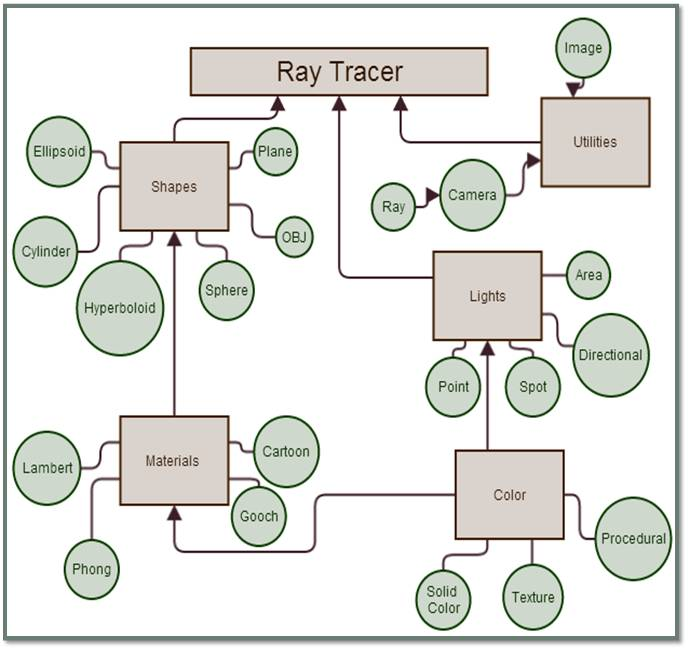
\includegraphics[height=3.0in]{figures/rayTracerStructure.jpg}
\caption{Diagram of the Parenting/Dependency Structure of the Ray Casting Program}
\label{fig:RayTracerDependencies}
\end{figure}
Preliminary preparations refers to anything that needed to be accomplished before being able to start coding the ray tracing theory coding.  In this section, simple matters such as program language installation and accessibility will be discussed.  Also discussed is the majority of the ``Utilities" section of Figure \ref{fig:RayTracerDependencies}.

The foundations of a ray tracing program are built around two fundamental procedures: image writing and vector math. Ray tracing can also be accomplished through matrix operations, but for the purposes of this thesis, vector math will be sufficient.  Vector math is the basis for all ray tracing theory. As such, a class or data structure that can accomplish all aspects of vector math including addition, subtraction, dot product, and cross product is crucial to accomplishing the image synthesis program.  In addition to this, in order to see the final product after all the calculations have been run, you must be able to write an image.  Arguably the easiest image file to write out is a Portable PixMap (PPM).  Other image formats include JPEG, BITMAP, and PNG.  Each of these image formats requires a more complicated compression algorithm than PPM.  Each programming language may also require additional files in order to compile or execute the final product.  Each of these languages will be assessed from the viewpoint of a student in the Visualization Department of Texas A\&M, because this is directly relevant to the my experience.
\subsection{C++}
The C++ language, as described in Section \ref{sub:C++}, is an object-oriented language that is considered both a high and low level language because of the level of control it provides over computer functionalities.  Development and installation with C++ was accomplished via the provided computers at Texas A\&M's Department of Visualization.

When developing in a Linux/Unix environment, C++ can be executed directly from the terminal of the operating system.  This means no external IDE is needed to compile your code.  This development environment was more appealing to me because IDE environments have their own learning curve, which would have to be realized in addition to learning the C++ language semantics.  If a Department of Visualization computer was not available, installation of the C++ development tools would present its own challenges.

To work on a Windows computer, you must first determine which compiler to work from, download that compiler, and then work from that specific compiler's commandline.  Common practice would be to download an IDE such as Visual Studio or Eclipse.  Since computers are not typically sold with a Linux operating system installed on them, developing in Linux outside of an academic setting would require installing a new operating system, which is not a task for beginners.  After learning how to install Linux, you must then learn the proper way to download specific compiler packages. Since this can be accomplished by simply typing a command into the computer's terminal, it can be significantly easier to learn how to do than installing a compiler on Windows.  A Macintosh computer was not tested, but since their operating systems are a variation of the Unix platform much like Linux, and since they are more commonly sold in stores, they are more accessible to students who are not computer scientists.  Starting to develop in C++ on any computer is a complicated task unless a ready-made environment has been provided for you, like at Texas A\&M.

What makes C++ unique from other languages explored in this thesis is the concept of a makefile, and the make command. In order to communicate with the compiler installed on the Unix platform, you need to create a file that will define which source code files are needed to make object files and which compilers and linkers are included in the make command.  A properly configured IDE it will automatically generate a makefile and perform the make command for you.  This further solidified my decision to work without a IDE and use a syntax highlighting text-editor, because nothing was generated automatically. That way, only what was typed and developed by myself was included in the project.  This allowed for easier debugging of the makefile and make command rather than debugging the IDE's internal processes.

The use of header files is another difference between C++ and the other languages used in this thesis..  When creating a class in C++, it is common practice to outline the class structure in one of these ``header" files. The header file serves as the skeleton of the class structure, while the meat of the class's implementation is fleshed out in a ``.cpp" file.  This is a technique inherited from C coding which was used for older computers that could not support large quantities of memory at the same time.  Computers have improved since and this antiquated practice now further segregates the interface of a class from the implementation of the class rather than save memory space during execution time.  For this thesis only header files were used since speed optimization was not a priority.

In addition to a makefile, another obstacle introduced by C++ was the vector math library.  C++ does not have a standard vector library: the operation needs to be hand-coded in order to be available for use.  A developer has to either implement their own vector math library or borrow a pre-existing library.  This requires additional research or work to write the necessary code.  If a developer is going to borrow code from the Internet, an assessment needs to be made regarding the original writer's accuracy.  Subsequently, knowledge must be gained on how to use the classes and structures defined in the borrowed library.  The vector class used for this thesis was a library circulating amongst the Texas A\&M students that was written by a former faculty member at A\&M: the know source is reputable and the code is trusted to be uselful and correct.

The same obstacle applies to the image reading and writing functionality of an image synthesis program.  There is no standard C++ image library.  Once again, in order to read and write images, a developer needs to either write their own code or borrow an existing third-party library.  For this thesis, a class was written to process .ppm images.  I decided that the effort required to create a custom class to process .ppm images would be less than the effort required to untangle the semantics of linking in a third-party image library.  The .ppm format was chosen because it was the most accessible and simplest format to implement.  The created images needed to be converted to .png or .jpg for use on the web and this was very limiting to the functionality of the final image synthesis program.  The thought of including a third-party library, more specifically the semantics of linking the files correctly in the coding process, seemed more difficult than writing an original class.
\subsection{Processing}
The programming language, Processing, approaches the preliminary preparation milestone in a manner that is significantly different from that of C++.  Whereas I was able to avoid IDE's for C++, doing so with Processing would have proven impossible as it happens to \textit{be} an modified and specially engineered IDE for the Java programming language itself.

Installation of the Processing language is simple.  A compressed application file is downloaded from the processing.org website. Once uncompressed an application file can be clicked and opened.  This starts the Processing application and development can begin.  The processing.org website provides downloads for the three major operating systems, Windows(32-bit and 64-bit), Linux(32-bit and 64-bit) and Mac OS X.  Processing does not require installation so it can be run from anywhere on your computer, which means that Processing can even be saved to, and run from, an external hard drive, allowing the developer to work from any computer without having to reinstall an IDE or compiler. The portability of Processing is convenient for students who may not have a laptop and are forced to switch between workstations.

Processing has a vector math library built into its IDE called PVector.  PVector has extensive documentation on the processing.org website.  Despite this, the syntax of PVector operations is anything but straightforward.  This can best be described with an example.  Consider the C++ equation for determining the hit point along a ray from the ray's origin:
\begin{equation}
\label{eq:C++Equation}
p_{hit} = ray.Origin + t*ray.Direction
\end{equation}

This same equation in PVector would be written:
\begin{equation}
\label{eq:PVectorEquation}
p_{hit} = PVector.add(cast.Origin, PVector.mult(cast.Direction,t))
\end{equation}

Rather than overload the math components of the Vector object, each operator is expressed as a function.  Thus, ``+" becomes ``add" and ``*" becomes ``mult.".  This leads Processing operations to grow long and segmented, which causes confusion for the programmer.  As can be seen in the above example, the C++ syntax in Equation \ref{eq:C++Equation} is much easier to read, understand, and therefore debug, than the Processing syntax in Equation \ref{eq:PVectorEquation}.

In addition to the PVector library, Processing also has included its own image library.  Unlike PVector this image library is very convenient, although no math operations were needed to be performed on image objects.  The PImage library has the ability to save or open any type of common image file, as long as the file type is specified within the command.

Processing introduced another challenge when dealing with color.  Color in Processing is defined as a data type, which is saved as 32-bits of data formatted as AAAAAAAARRRRRRRRGGGGGGGGBBBBBBBB, where (A)lpha, (R)ed, (G)reen, and (B)lue components are all stored as 8 bits of data. Within a ray tracer it is necessary to have access to each individual color value in order to take color averages, since you need to calculate each color value individually.  To extract each color value from the color type a process called bit shifting must occur. This can be shown as follows(example taken from processing.org):

\singlespacing
\begin{lstlisting}[language=Java, caption=Java bit shifting to extract color data, style=mystyle, label=list:javaBit]
color argb = color(204, 204, 51, 255);
int a = (argb >> 24) & 0xFF;
int r = (argb >> 16) & 0xFF;  // Faster way of getting red
int g = (argb >> 8) & 0xFF;   // Faster way of getting green
int b = argb & 0xFF;          // Faster way of getting blue
\end{lstlisting}
\doublespacing
Bit shifting is a technique that exposes the base functionality of how computer's save information within their internal storage. The process of bit shifting is not trivial and is confusing for new programmers who are unfamiliar with computer architecture.  As can be seen by Figure \ref{list:javaBit}, Processing has made available information and resources to solve some of the more complicated challenges introduced by the Java language.

\subsection{Python}
Many of the same complications that arise with C++ also occur with Python.  Like C++, Python does not have a vector math library built in.  It is also rather complicated to install correctly on a Windows machine.

Unlike C++, however, header files are not necessary for Python programs, nor do the programs have to be compiled before running.  Python also comes pre-installed on Unix-based systems so development can begin right away on Linux and Macintosh computers.  Running a Python program can be done through the computer's terminal in much the same way as C++.

Although Python does not have a vector math library, I found it easier to find third party vector libraries written in Python. This might be to due to the surge of popularity that the Python language has experienced over the past few years.  For this thesis, a vector library was written using the C++ vector library as a template.  The decision to write an original Python vector library rather than using a pre-existing library was made to take advantage of an educational exercise that would help familiarize me with the Python language.

The imaging library that was used for this thesis is called the Python Imaging Library(PIL).  PIL was originally a Python-supported library until their most recent release.  PIL is now a third party image library that is still under development.  PIL is only compatible with Python version 3.0 or earlier, so if a later version of Python is used PIL cannot be included in the project. It is recommended to avoid writing a custom image library and instead to use a version of Python that supports PIL because it is more beneficial to have the PIL capabilities rather than write a image class from scratch.
\subsection{RenderMan\copyright}
Compared to the other three programming languages in this thesis, RenderMan\copyright \space is an outlier.  It does not follow the same milestones as the other coding languages  which may appear to be a huge advantage, but there is a major drawback.  RenderMan\copyright\space is a very expensive rendering engine that is not available to the average computer graphics hobbyist.  As of the writing this thesis in 2014, a RenderMan\copyright\space Floating Institutional license sells for \$274.00.  The same is true for a Pro Server license.  A one year student subscription costs \$199.95 and does not allow students to produce anything for commercial value.  The yearly cost times four years of schooling equates to \$800 on top of tuition and other expenses.  It is not in my budget, nor in the typical students' budget, to have access to RenderMan\copyright\space outside of an academic setting.  Thankfully Texas A\&M has an Institutional license for RenderMan\copyright\space that was used for this thesis.  This cost ranked RenderMan\copyright\space lowest of all the languages for accessibility and portability.

It is worth noting that there is an open source alternative to RenderMan\copyright\space called Pixie\copyright.  Pixie\copyright\space is based off of the RenderMan\copyright\space syntax but does not have all of the same features that RenderMan\copyright\space does, nor was it developed by the same people at Pixar.  If learning the RenderMan\copyright\space syntax and RIB/RSL file structure is desired however, then Pixie\copyright\space is an affordable alternative to use from home or outside of an academic environment.

\section{Milestone 2: Direct Illumination- Ray Casting}
A majority of the planning and learning involved in this research occurred on an implementation level during this second milestone because it was the first milestone to implement code.  Declaring a class was a different learning experience for each language.  C++ and Processing have a similar syntax but Python is different both in syntax and in theory.

A class is fundamentally a descriptor of characteristics and behaviors needed by a virtual ``object" in a computer program.  Class declaration and planning for each language is important because they relate back to accomplishing the ray-tracing theory. The goal, remember, is to determine which object, if any, intersects with each pixel in an image. This is done by iterating over every object in a scene to determine if it intersects with the pixel in question.  The goal is to have all of the data storing each object in the scene held in one place so that only one iteration loop needs to be written. Since it is unknown how many objects are in a scene at one time, the container size for holding the data for the objects needs to be dynamic in size.  This introduces the two main challenges for implementing basic ray casting theory in a computer program: organization of classes(objects) and assembly of those classes into a dynamically-sized data container (or data structure).
\subsection{Classes Overview}
In order to successfully determine how classes should be established, it is important to plan how classes should relate to one another.  The relationships of one class to another can most successfully be summarized in Figure \ref{fig:RayTracerDependencies}, found in Section \ref{Milestone1}.  The picture represents the four main object types: \textbf{shapes}, \textbf{materials}, \textbf{color}, and \textbf{lights}. In summary, every \textbf{shape} must have a \textbf{material}, which must have at least one \textbf{color}.

The different types of \textbf{shapes} are represented by the circles sprouting locally around its pink square (sphere, ellipsoid, cylinder, etc..), just as the type of \textbf{material} can be any of the circles sprouting from its pink square (Lambert, Phong, Cartoon).  The circles represent child classes.  Child classes can inherit the properties and behaviors of their parent class. \textbf{Lights} do not have any connection with \textbf{shapes} or \textbf{materials}, but each \textbf{light} must have a color, which then provides color information for a material.  Classes can be broken into two main elements: variables, which hold data within the class, and functions, which modify the data that is held within the class.  In all languages variables have a specific type, for instance integers (whole numbers), floats (decimal numbers), and strings (words or letters).  Defining custom classes is a way the programmer can introduce new variable types. The following is an abstract summary of each of the primary variables and functions for each major class type established in this raytracer program. For simplicity sake we will just discuss the functions vital to basic ray casting theory, rather than any extra helper functions that might have been implemented.
\subsubsection{Shapes}
The shape parent class consisted of four variables and three functions. The class structure is demonstrated in the Unified Modeling Language (UML) diagram, Figure \ref{uml:shapeclass}, below.

\begin{figure}[ht]

\centering
\includegraphics{class_diagram.1}
\caption{Unified modeling language \(UML\) Diagram for the Shape Class}
\label{uml:shapeclass}
\end{figure}

As shown above, the shape class had all the important base functionality for every shape object.  Associated with every shape object was a vector object that described its position in 3D space (Position), a Vector that was calculated to describe where a light ray or camera view ray would hit the shape (Hit Point), a material object that described what the shape would look like when interacting with the light and camera view vectors (Material), and a distance integer that helped to sort all the shapes in the scene from closest to farthest away(distance).  The shapes initially had three important base functions that calculated the following: if the shape intersected a light ray (intersect); what material on the object the return color would be based off of(rtnColor); and the surface normal that was given from the intersection point (calcNormal).  These three functions were inherited by all of the children shape objects.

\subsubsection{Color}
The color parent class incorporated all types of color information that could be displayed in a material.  The color objects were vectors that held Red, Green, and Blue(RGB) hue information with the ability to be added and subtracted from each other.  Color information could also be taken from an image or a procedural equation to describe the RGB information transmitted from the surface. Figure \ref{uml:colorclass} shows the color class.

\begin{figure}[ht]
\centering
\includegraphics{class_diagram.3}
\caption{UML Diagram for the Color Class}
\label{uml:colorclass}
\end{figure}
The color parent object held Color information in a Vector (RGB) and a method that described how to calculate the color vector(returnColor()).

\subsubsection{Materials}
\begin{figure}[!ht]
\centering
	\includegraphics{class_diagram.2}
\caption{Unified Modeling Language Diagram displaying important Material Class features}
\label{uml:materialclass}
\end{figure}

As can be seen from Figure \ref{uml:materialclass}, the material class very simply had a variable that stored a color object (Color), which described which color would be used when calculating the returned color from the returnColor function.  This variable was either overwritten or added onto in child classes, but the base material parent class was used as a holder for all material objects.
\subsubsection{Lights}
A light object was very simple and followed the UML Diagram in Figure \ref{uml:lightclass}.
\begin{figure}[!ht]
\centering
\includegraphics{class_diagram.4}
\caption{Unified Modeling Language Diagram displaying important Light Class features}
\label{uml:lightclass}
\end{figure}
A parent light object held only the information needed to determine the color for the light so the variables were the color object and position vector. The function calculated whether or not the light intersected with the object and if so, the color that would be returned from the light's color object.

\subsection{Declaring Classes with each Language}
For this section, we will use the Shape class to demonstrate how classes are declared in each language.  The Shape class structure is defined in figure \ref{uml:shapeclass}.
\subsubsection{C++}
\singlespacing
\begin{lstlisting}[language=C++, caption=C++ Class Example, style=mystyle, label=list:c++Class]
//  Shape Class
#ifndef SHAPE_H
#define SHAPE_H

#include "../classes/Vector.h"            //Vector class
#include "../materials/material.h"        //Material class
#include "../lights/light.h"              //Light class
#include "../utils/ray.h"                 //Ray class
#include <iostream>
#include <string>

using namespace std;

class Shape
{
  protected:
    Vector3d position;
    Material *mat;
  public:
    Vector3d hit_point;

    //constructor
    Shape(){
      position = Vector3d(0,0,0);
      mat = new Material();
      cast = true;
      blur = false;
    };
    Shape(Vector3d pos){
      position = pos;
      mat = new Material();
    };
    ~Shape(){};
    //function to return the Color Vector returned
    //from a light ray intersection on with the material
    virtual Vector3d matReturn(Ray ray, Light *light)
    {
        return mat->rtnColor();
    };
    //function to determine hit_point and return
    //boolean to determine if surface of object was hit.
    virtual bool intersect(Ray cast){
        //calculate if ray intersects object's position here...
    };
};
#endif
\end{lstlisting}
\begin{lstlisting}[language=C++, caption=C++ Class Usage Example, style=mystyle, label=list:c++Use]
Sphere sphere_object = new Sphere();
//if ray object was created we can pass the object into the intersect function.
bool is_hit = sphere_object->intersect(ray_object);
\end{lstlisting}
\doublespacing
\subsubsection{C++ Explained}
The C++ declaration of a class has a few quirks that are different from other languages.  One: ``include guards" (found on lines two and three of Listing \ref{list:c++Class}).  An include guard prevents the Shape.h class from being defined multiple times, which can happen if Shape.h is included, or referenced, into multiple classes within the ray tracing program, especially within classes that inherit from each other.   Include statements are found on lines five through ten of Listing \ref{list:c++Class}. Inclusion of these has the potential to cause an error and inhibit the program from running.  It can be argued that every class can be written in one extremely long document and remove the need for include guards and include statements, but this will create a document that is difficult to debug and troubleshoot when errors occur. Determining all the needed include statements when creating a class for the first time can be tricky and forgetting to include necessary classes will cause an error.

Line twelve demonstrates a standard practice in C++ that describes in which context the file can be used, which in C++ is called a namespace.  For the sake of simplicity, all files in this project use the standard, or std, namespace.

The declaration of the class begins on line fourteen.  The keyword ``class" followed by the name of the class and curly brackets signifies the start of a class.  Within the brackets variables can start to be declared and and the functions necessary to the shape class.  Line sixteen begins the declaration of class variables.  Variables can be defined in one of three groups in C++: public, protected, or private.  The protected variables that are declared on line sixteen can only be accessed by classes that inherit from the shape class.  The public variables declared on line nineteen can be accessed from any program that creates a shape object.  As can be seen, we have grouped each variable and function inside of a ``protected" (line 16) and a ``public" grouping (line 19).  For this thesis, most variables were considered private or protected, but there is no issue with leaving all variables public.  Public, protected, or private variable scope needs to be considered when trying to create an object-oriented ray-tracer.  Having protected variables allows for more confidence in the values of variables staying exact because access to the variables is limited to methods provided within the class.

Next in the figure is the constructor on line 23 and 29.  A constructor is a required function that instantiates a class.  Without a constructor line 1 of Listing \ref{list:c++Use} would not be possible.  Constructors are defined like other functions but with a name that matches the class name.  Two constructors are defined as a shortcut to setting the internal variables of a class.  Line 29 allows the creation of a shape class at a specified coordinate as opposed to 0.0, 0.0, 0.0.  Following the constructor are the functions that are used to calculate various important information.  Since the functions defined on line 36 and line 42 are grouped under the ``public:" section of the class, these functions can be called as elements of the class after they have been instantiated.

To declare a C++ function the scope needs to be determined, the variable type that will be returned declared, and the function named. On line 42 of Listing \ref{list:c++Class} we declare a public function(because of the public grouping earlier in the code) that returns a boolean, or true/false value, in a function called ``intersect". The \textit{virtual} keyword is discussed in later sections.

All of these components need to be considered when declaring a class with C++.  If any of these things are not correct a variety of errors can be occur that need to be handled before the ray tracer will complete.

\subsubsection{Processing}
\singlespacing
\begin{lstlisting}[language=Java, caption=Java Class definition example, style=mystyle, label= list:javaClass]
/*
  Abstract Shape Superclass encompassing all shape objects
*/
abstract class Shape{
  //Global Variables
  PVector hit_point;  //hit point on the surface of the object

  //Protected variables only to be used by Shape subclasses
  protected PVector position;  //position of the Shape in 3D space
  protected Material mat;  //Material assigned to this shape

  //Basic Shape constructor
  Shape(){
    position = new PVector(0,0,0);
  }

  //Another Shape Constructor
  Shape(PVector pos){
    position = pos;
  }

  //Another Shape Constructor
  Shape(PVector pos, PVector up){
    position = pos;
  }

  //function to return the Color Vector returned
  //from a light ray intersection on with the material
  PVector matReturn(Ray ray, Light light)
  {
    return mat.rtnColor();
  }
  //function to determine hit_point and return
  //boolean to determine if surface of object was hit.
  boolean intersect(Ray cast)
  {
    //calculate if ray intersect's objects position here...
    return true;
  }
}
\end{lstlisting}
\begin{lstlisting}[language=Java, caption=Java Class definition example, style=mystyle]
Sphere sphere_object = new Sphere();
bool is_hit = sphere_object.intersect(ray_object);
\end{lstlisting}
\doublespacing

As nas been shown, Processing class declarations have some similarities to C++ classes but also have some differences.  Unlike C++, Processing does not require any include guards or include statements.  Including is accomplished by the Processing IDE.  All tabs that are open within the Processing ``sketch" are included and available to every other file within the project.  Ignoring the abstract keyword for now, line four of Listing \ref{list:javaClass} is the same as C++.  Processing follows the constructor format of C++ as well.  A difference between C++ and Processing is the variable scope declarations.  In C++, variables and functions were grouped under ``public:" and ``protected:" tags. With Processing, however, each variable must be individually declared \textit{not} public, which is the default scope declaration, as can be seen on lines 10 and 11.

\subsubsection{Python}
\singlespacing
\begin{lstlisting}[language=Python, caption = Example of class definition in Python, style=mystyle, label=list:pyClass]
"""##########################################################
  Shape.py File
##########################################################"""
import sys, math
import Vector, Material, Ray

class Shape(object):
  __slots__ = ('hit_point', 'position', 'mat')

  #constructor
  def __init__(self, position = Vector.Vector3d(0.0,0.0,0.0)):
    self.position = position
    self.mat = Material.Material()

  #function to determine hit_point and return
  #boolean to determine if surface of object was hit.
  def intersect(self, cast):
    #calculate if ray intersects object's position here...
    return true

  #function to return the Color Vector returned
  #from a light ray intersection on with the material
  def matReturn(self, ray, light):

    return self.mat.rtnColor()

\end{lstlisting}
\begin{lstlisting}[language=Python, caption=Python Usasge Example, style=mystyle,label=list:pyUse]
sphere = Sphere.Sphere();
is_hit = sphere.intersect(ray_object);
\end{lstlisting}
\doublespacing

Python is the most different from C++ and Processing.  While the other two languages separate blocks of code using curly braces, Python uses white space to define its code structure, so function and variable scope are determined by tab depth and the colon(``:") character.  This was a big hindrance in development of code because the scope of each for-loop or function needed to be perfect, and if code blocks are not highlighted by a text editor, the Python indent can get confusing and lead to code working improperly.  To create a class in Python, include statements like C++ must be used, as can be seen in Listing \ref{list:pyClass} on line 4 and 5.  Include guards, however, do not need to be used.  Python's keyword for include is ``import".  Utilizing the imported classes is different than in C++ or in Processing.  As can be seen on line 13, in order to use any methods from the imported class the function or variable name must be prefixed with the name of the import class it is being taken from. In this case, the constructor function from the imported Material class is used with Material.Material().  Declaring a class on line 7 is the same as with C++ or with Processing, the exception being that within the parentheses it needs to be specified what the class inherits from.  The default is object, because all classes are objects.

One way to declare class variables within a Python class is the ``\_\_slots\_\_" notation, which is found on line 8.  This is a more advanced technique that will save space within the final implementation process, but is not always necessary.  An effort was made to try to get Python classes to look as similar to their C++ and Processing counterparts within the context of the thesis.  Normally within Python, variables can be declared and added to a class from anywhere after a class has been instantiated.  Slots limit the number of available variables to specific variable names, which saves memory in the long run but also prevents extra or unwanted variable declarations within instantiated objects.  The concept of variable scope in Python is foreign.  To accomplish protected or private variables in classes follow a convention called ``name mangling", which simply adds at least one underscore before a variable name. This, however, does not cause the variable name to act protected or private; it just makes it harder to guess what the variable name is when trying to access it from another application that is instantiating a python object.  For this thesis, the Python ray caster used only public variables.

The method for declaring a constructor in Python is also different.  The constructor syntax for Python can be seen on line 11.  Python easily allows for declaration of a constructor.  Unlike C++ and Processing, all Python functions require the ``def" keyword to establish them as functions.  Whereas in C++ and Processing a function with the same name as the class declares a constructor, the distributed keyword \_\_init\_\_ function is the constructor argument for the Python class.  Classes are still instantiated with a function that mimics the class name, however, as is seen in Listing \ref{list:pyUse}, line 1.  As in every Python function, the first argument provided to the function must be ``self", which allows the Python function access to its own information.  The self keyword is demonstrated in line 12 within the constructor where the position variable passed into the function is set to be self.position, which refers to the position variable established within the \_\_slots\_\_ array.  Without a reference to ``self", the constructor would have no access to any of the class variables.  The self keyword is Python's way of handling scope.  The second argument, ``position = Vector.Vector3d (0.0 ,0.0 ,0.0)", eliminates the need for a second constructor because this sets a default for the position argument of the constructor if no value is provided when the constructor is instantiated.  This accomplishes the same thing that was done in Listing \ref{list:c++Class} line 23 and line 29.

\subsection{Dynamic Class Variables}
Since Processing and C++ are both static-typed languages, a unique challenge occurs.  Line 18 of Figure \ref{list:c++Class} and line 10 of Figure \ref{list:javaClass} shows that avariable of type material has been declared.  This means that only a class that is instantiated as a material object type can be saved as that object's variable.  Theoretically, however, a shape class to have an infinite range of material objects that are not strictly Material classes, but rather also a lambert object, phong object or even cartoon type, that are an instance of a Material class, but still have the same properties as the Material class.  If an attempt was made to create a phong object and save it within a shape object as the mat variable, this would not work and cause an error upon compilation.

To give some insight as to why each language was designed this way, Cardelli and Peter describe strong-typed, or static-typed, languages in their article entitled \textit{On Understanding Types, Data Abstraction, and Polymorphism} as follows:
\begin{quote}
Static typing allows type inconsistencies to be discovered at compile time and guarantees that executed programs are type-consistent. It facilitates early detection of type errors and allows greater execution-time efficiency. It enforces a programming discipline on the programmer that makes programs more structured and easier to read. \cite{cardelli1985understanding}
\end{quote}

Eliminating this data type issue is not possible but there is a solution to saving a phong object as a material variable. Two computer science terms called \textit{inheritance} and \textit{polymorphism} help to solve this problem.  Inheritance is the idea that a child class can inherit the properties and functions of a parent class.  Making a phong object a child of a material object, enables the phong object to be saved as a material variable within the shape class without throwing an error. This is accomplished in C++ as follows:

\singlespacing
\begin{lstlisting}[language=C++, style=mystyle, label=c++Inherit]
//material.h file//
class Material
{
    public:
        Material(){};   //constructor
        Color color;
        virtual float returnColor(){
            //calculate material color for shape hit point
        }
}
\end{lstlisting}
\begin{lstlisting}[language=C++, style=mystyle]
//phong.h file//
#include "phong.h"
class Phong: public Material
{
    public:
        Phong(){};  //constructor
        Color color2;   //new color variable specific to phong class.
        float returnColor(){
            //calculate sphere size logic.
        }
}
\end{lstlisting}
\begin{lstlisting}[language=C++, caption=C++ Inheritance Example, style=mystyle]
//lambert.h file//
#include "lambert.h"
class Lambert: public Material
{
    public:
        Lambert(){};
        Color color2;
}
\end{lstlisting}
\doublespacing

In the above example, all classes have at least one Color variable and a returnColor() function because of inheritance. The Lambert/Phong classes each have two variables because they establish another Color variable (color2) within themselves and inherit the Color variable from the parent material class.  The returnColor() function for the material and lambert classes will function the same but the phong's have different logic because the logic has been overwritten(for this example, for the thesis the lambert class also overwrites this function).

All children classes need to call their own constructors in order to be instantiated.  It is important to note that a child class must contain ``\#include `material.h'" or it will not work correctly. In order to rewrite a parent function in a child class the keyword ``virtual" needs to be used as seen on the returnColor() function(line 9) in Figure \ref{c++Inherit}.  To accomplish this same procedure in Processing, classes need to be established as follows:

\singlespacing
\begin{lstlisting}[language=Java, style=mystyle]
//material.pde file//
abstract class Material
{
    Material(){};  //Constructor
    protected Color color;
    float returnColor(){
        //calculate size for all object types;
    }
}
\end{lstlisting}
\begin{lstlisting}[language=Java, caption=Java Abstract Class Example, style=mystyle, label=javaInherit]
//phong.pde file//
class Phong extends Material
{
    Phong(){};
    protected Color color2;
    float returnColor(){
        //calculate size specific for sphere
    {
}
\end{lstlisting}
\doublespacing
The syntax for the cube.pde file is the same as the sphere.pde with the ``extends" keyword showing that the sphere is the child of the Shape class.

Inheritance only achieves half the goal. If the above Phong and Material classes were implemented and then instantiated and finally saved as a phong object type within the material variable within the shape object, all variables and functions written specifically for the phong class will be discarded and replaced by the functionality of the parent class.  We will be virtually shaving off the corners of the square ``phong" peg to fit it back into the circle ``material" hole that has been prepared for it within shape objects storage in memory.  This can be avoided with polymorphism.

Cardelli and Wegner explain different types of polymorphism, from which the type used for this thesis is called subtyping.
\begin{quote}
Subtyping is an instance of \textit{inclusion polymorphism}. The idea of a type being a subtype of another type is useful not only for subranges of ordered types such as integers, but also for more complex structures
such as a type representing Toyotas which is a subtype of a more general type such as Vehicles. Every object of a subtype can be used in a supertype context in the sense that every Toyota is a vehicle and can be
operated on by all operations that are applicable to vehicles. \cite{cardelli1985understanding}
\end{quote}
To introduce how this is achieved in each language, the topic of ``pass-by-value" and ``pass-by-reference" must be discussed.  In C++, when declaring an object, two variations can be done in relation to the memory organization within the computer.  The first, ``pass-by-value", is the most common and every time a variable changes or moves a \textit{copy} of the variable is made within the backend and saved in a new location.  However another schema, ``pass-by-reference" exists, however, which creates a reference or ``pointer" back to the original variable rather than copying the data.

Subtyping will allow us to ``pass-by-reference" our phong objects into a material variable and still retain the phong-specific information.  Subtyping and how it is used is also relevant to our second main challenge for implementing basic ray casting theory: assembly of classes into a dynamically-sized data container (or data structure).

\subsection{Data Structures}
\begin{figure}[ht]
\centering
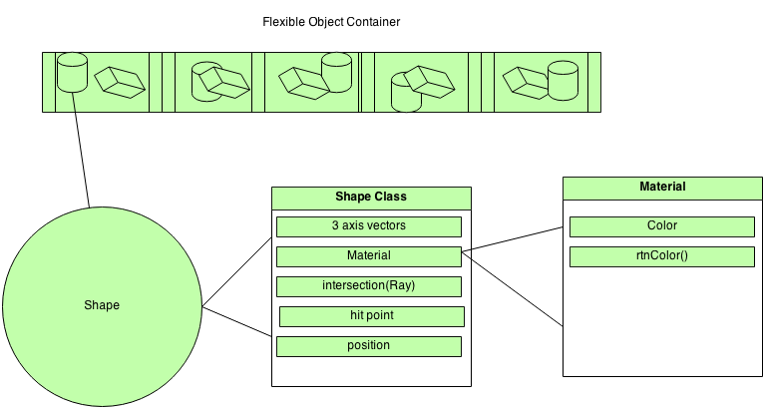
\includegraphics[height=3.0in]{figures/data_structure.png}
\caption{Data structure design for each program}
\label{fig:RayTracerDataStructure}
\end{figure}

It is more difficult to accomplish the data structure task in C++ and Processing (Java).  Just as a variable must be of the same type to save it to a class, all objects must be of the same type to add them to a data structure.  Furthermore, the most basic data structure, an Array, must be declared a specific size upon initialization.  The size issue can be easily circumvented, however.  For each language there is a dynamic container that will grow and shrink in size. C++ has a vector data structure and Processing has an ArrayList. To declare each is simple:
\begin{lstlisting}[language=C++, caption=C++ Vector Example, style=mystyle]
vector <Sphere> sphere_list;
Sphere sphere_object = new Sphere();
sphere_list.push_back(sphere_object);
\end{lstlisting}
\begin{lstlisting}[language=Java, caption=Java ArrayList Example, style=mystyle]
ArrayList<Sphere> sphere_list = new ArrayList<Sphere>();
Sphere sphere_object = new Sphere();
sphere_list.add(sphere_object);
\end{lstlisting}
Each of the above examples creates a \textit{Sphere} list, an instance of a \textit{Sphere} object, and subsequently puts that \textit{Sphere} object into the \textit{Sphere} list.  Note that each structure \textit{must} be declared as the type of object that is being placed into it. The ``pass-by-reference" tactic in C++ is what allows different variable types to be saved to a common parent data structure, as follows:
\begin{lstlisting}[language=C++, caption=C++ Vector Example, style=mystyle]
vector <Shape*> shape_list;
Shape *sphere_object = new Sphere();
Shape *cube_object = new Cube();
shape_list->push_back(sphere_object);
shape_list->push_back(cube_object);
\end{lstlisting}
Declaring the vector with the ``*" denotes a C++ pointer, or that the variable will use the ``pass-by-reference" schema.  Pass-by-reference and pass-by-value variables cannot be combined within a data structure.  To then call any functions within the pointer variables, ``-\textgreater" must be used rather than ``.".  This allows for all shape objects to be saved within the same data structure.

To accomplish this in Processing the Shape class was declared as abstract in Figure \ref{list:javaClass}.  This keyword signifies that an object of this type may not be instantiated within a program.  This keyword demonstrates true inheritance because it acts as a placeholder for commonly used functions and variables between class types.  In Java, it allows child classes to be declared as common types without losing each class's individual functions and variables. This is accomplished as follows:
\begin{lstlisting}[language=Java, caption=Java ArrayList Example, style=mystyle]
ArrayList<Shape> shape_list = new ArrayList<Shape>();
Shape sphere_object = new Sphere();
Shape cube_object = new Cube();
shape_list.add(sphere_object);
shape_list.add(cube_object);
\end{lstlisting}
\doublespacing
Notice that sphere\_object and cube\_object are declared as a type shape but using the child class's individual constructors.  This allows ``shape\_list.add()" to be called on the next two lines without throwing an error.  If the Shape class was not declared as abstract, when declaring Shape sphere\_object and calling the child constructor, and when calling functions that are specific to the child class, those calls will be replaced with calls to the parent class's functions.  

While Java still has ``pass-by-value" and ``pass-by-reference", Processing/Java has simplified their language to effectively make all declared variables function as pointers, pointing back to the original variable declaration.

\subsection{Python Inheritance and Data Structures}
While parent classes are not important for Python list functionality because Python is considered a dynamically-typed language (as opposed to the static-type for C++ and Java), for organizational purposes they were used and inheritance was declared as follows (note tabs and spacing), using the same example:

\singlespacing
\begin{lstlisting}[language=Python, style=mystyle]
//shape.py file//
class Shape(object):
    __init__(self,...):
        //shape constructor
    def size(self,...):
        //size calculation for all child classes
\end{lstlisting}
\begin{lstlisting}[language=Python, caption=Python Class Inheritance Example, style=mystyle]
//sphere.py file//
import Shape
class Sphere(Shape.Shape):
    def __init__(self,...):
        //sphere constructor contents
    def size():
        //calculate size specific for sphere
\end{lstlisting}
\begin{center}
\line(1,0){100}
\end{center}
\doublespacing
\subsubsection{Data Structure}
Accomplishing the data structure task in Python is the most simple and takes no extra effort.  Simply declare an object and place it in a Python list, like so:
\begin{lstlisting}[language=Python, caption=Python List Example, style=mystyle]
sphere = Sphere.Sphere();
cube = Cube.Cube();
objects =  [];
objects.append(sphere);
objects.append(cube);
\end{lstlisting}
The above code creates a sphere object, cube object, and an objects list, then adds the sphere and cube into the data structure with the lists append method.  Python lists can accept any combination of different variable types, which can be useful for a ray-tracers implementation but dangerous for software prosperity and robustness.  If the assumption is that all variables in a list have the same type and therefore the same associated functions, when an object that does not fall under these assumptions gets added to the list the program will fail.  More care needs to be taken to make sure all variables are of the correct type that are added to a list to ensure that the program will run successfully, since this is not required for the program to initially start running.

\subsection{Milestone Results: Processing Time Overview and Images}
Once the issues with class and object declaration were solved implementing the Basic Ray Casting Milestone was very straightforward with each language.  There was one issue with the Processing language, however, that accounted for a majority of the Processing implementation and accounts for a core theory of ray tracing implementation.
\subsubsection{Left Hand vs. Right Hand Rule}
In the 3-D virtual world there is a set of governing rules that determine an object's position within the space, known as a coordinate plane.  As in a two dimensional graph, a 3D scene contains an X and Y coordinate, but a new coordinate, Z, is added.  The order and direction for each of these axes, as they're called, determines many important calculations when determining size and space of objects in the scene.  Left-handed and right-handed can be described as follows(from processing.org):

\begin{quote}
``In order to draw something at a point in three dimensions the coordinates are specified in the order you would expect: x, y, z. Cartesian 3D systems are often described as ``left-handed" or ``right-handed." If you point your index finger in the positive y direction (up) and your thumb in the positive x direction (to the right), the rest of your fingers will point towards the positive z direction. It's left-handed if you use your left hand and do the same."
\end{quote}
For the C++ and Python implementations of the ray tracers a coordinate system needed to be created from scratch. I am right handed and therefore a right-handed coordinate system was used.  This means, when looking at a computer monitor, the positive Y axis points towards the top of the screen, the positive X axis points to the right of the screen and the negative Z axis points directly out of the screen, perpendicular to the screen's surface.  This is not a typically traditional schema for coordinate planes with computers, nor is it the scheme used by Processing.  Processing used a left-handed coordinate system where the positive y axis points towards the bottom of the screen, the positive X axis points towards the right of the screen, and the positive Z points away from the user, towards the back of the computer, perpendicular with the computer screen.  Many of the calculations associated with cross products and other vector math needed the Y value and Z value negated so that the caluclations behaved more similarly to the other two ray tracing programs.
\subsection{Basic Ray Casting Images}
Here are a few images from the Basic Ray Casting Milestone.  While these are just a few examples from each language and each task, each language accomplished the same types of images that are presented in Figures \ref{fig:processingraycasting} through \ref{fig:processingtriangles}.
\begin{figure}[ht]
\centering
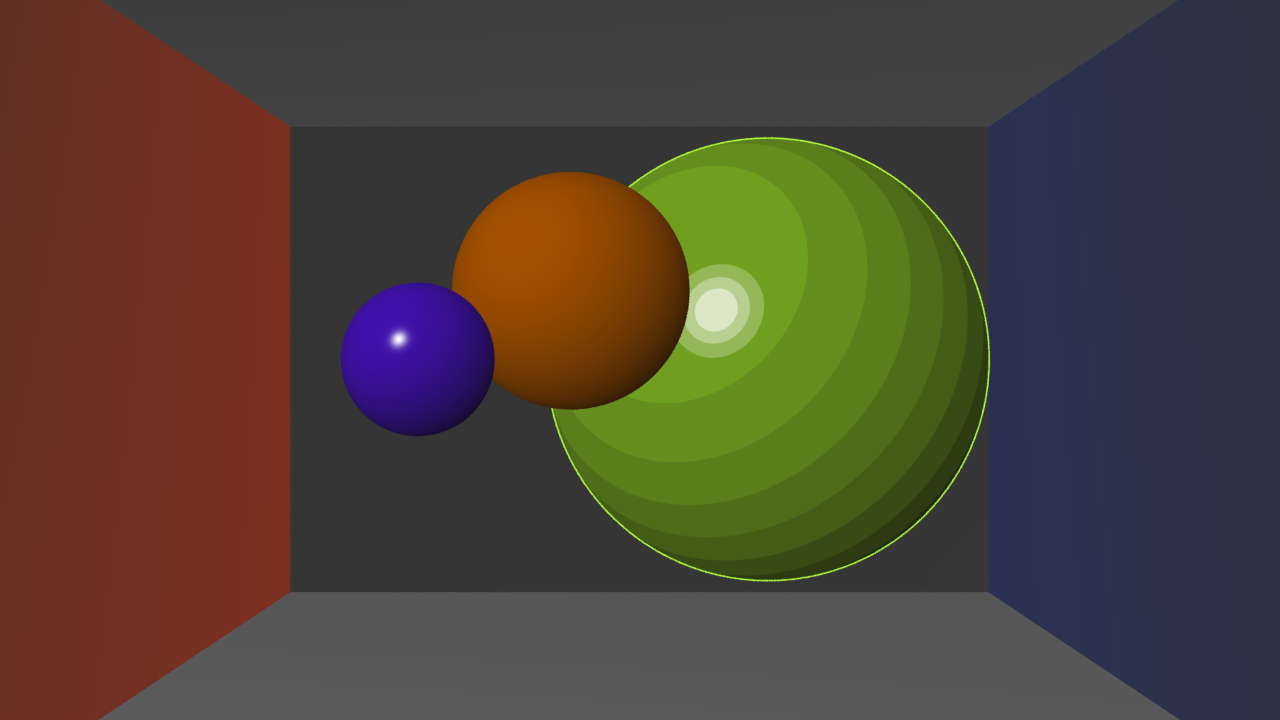
\includegraphics[width=\textwidth]{figures/BasicRayCastingProcessing.png}
\caption{Ray Casting Accomplished with Processing. Shown are three spheres with a different texture type for each, and five planes all with flat textures applied.}
\label{fig:processingraycasting}
\end{figure}

\begin{figure}[ht]
\centering
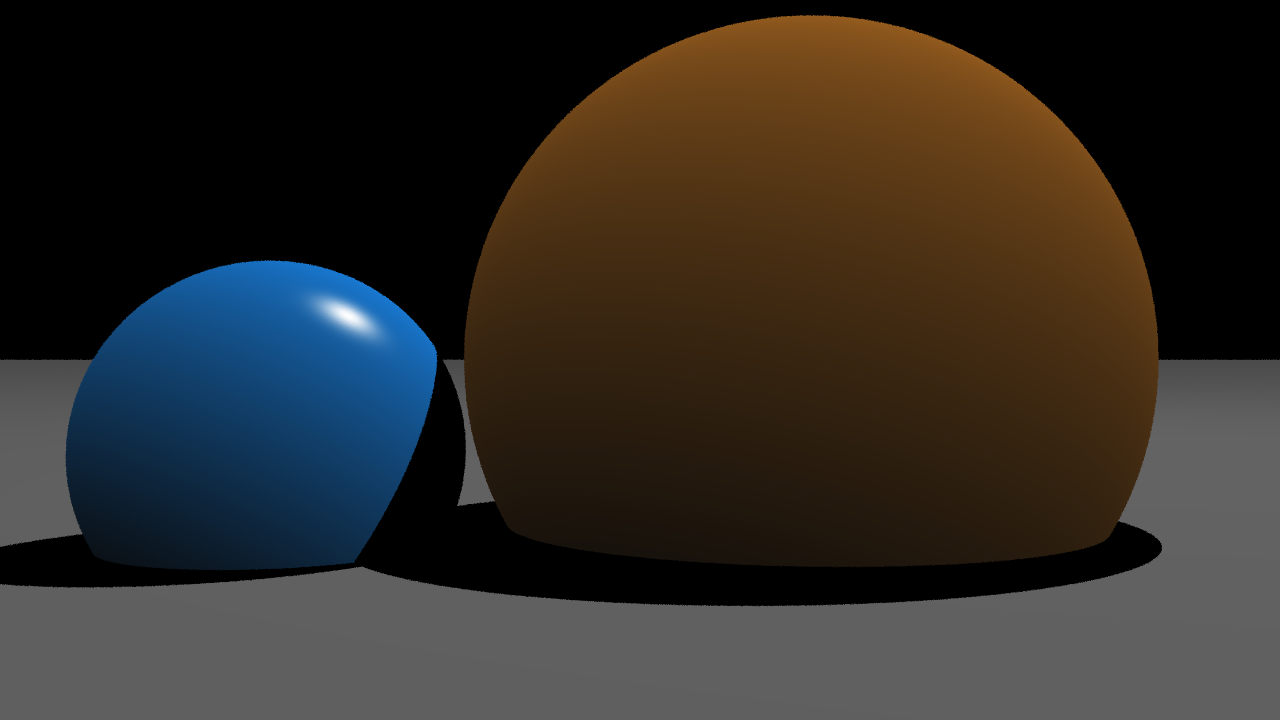
\includegraphics[width=\textwidth]{figures/ShadowCastingPython.png}
\caption{Ray Casting Accomplished with Python.  Shown are two spheres, and one plane that all cast shadows from a simple point light. }
\label{fig:pythonraycasting}
\end{figure}

\begin{figure}[ht]
\centering
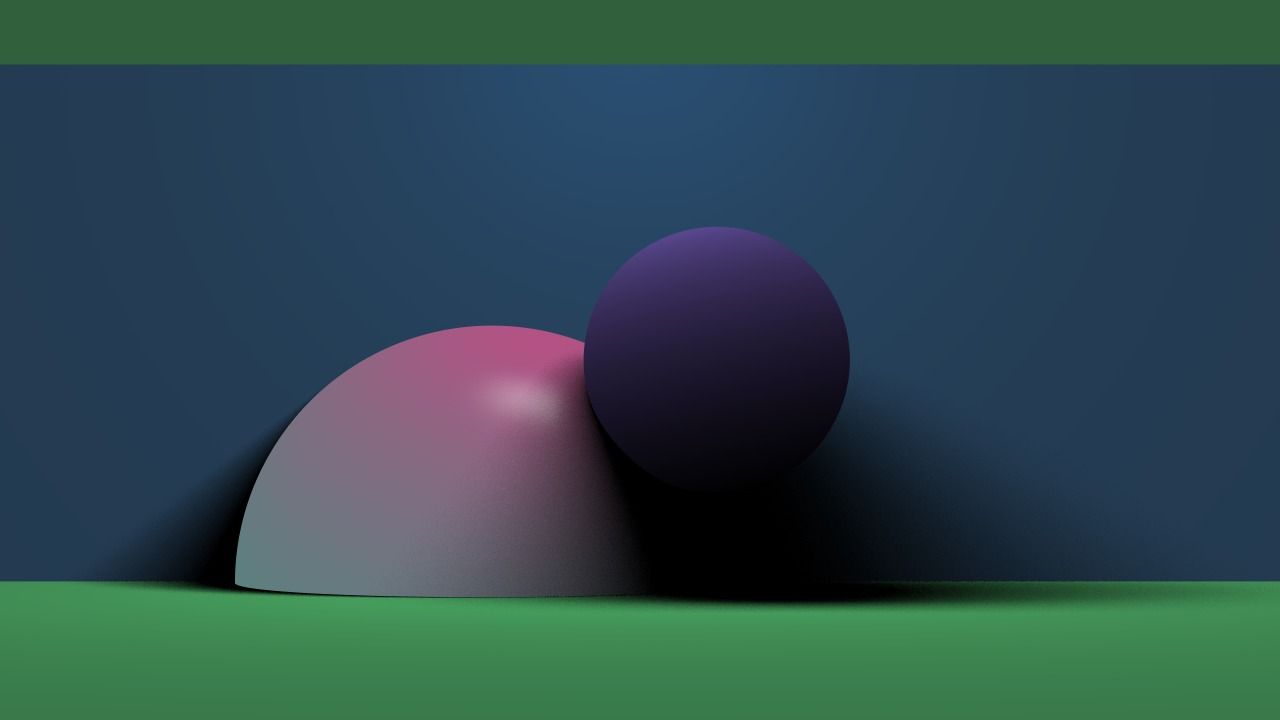
\includegraphics[width=\textwidth]{figures/ShadowCastingC++.jpeg}
\caption{Ray Casting Accomplished with C++.  Shown are two spheres, five planes and an area light that all cast shadows, which accounts for the soft shadow effect. }
\label{fig:cplusraycasting}
\end{figure}

\begin{figure}[ht]
\centering

\includegraphics[width=\textwidth]{figures/texturingC++.jpg}
\caption{Ray Casting Accomplished with C++.  Shown are two spheres with 2 separate shader types with two separate images mapped to them, and two planes, one with a repeated image texture and one without any image texture. }
\label{fig:cplusraycasting}
\end{figure}

\begin{figure}[ht]
\centering
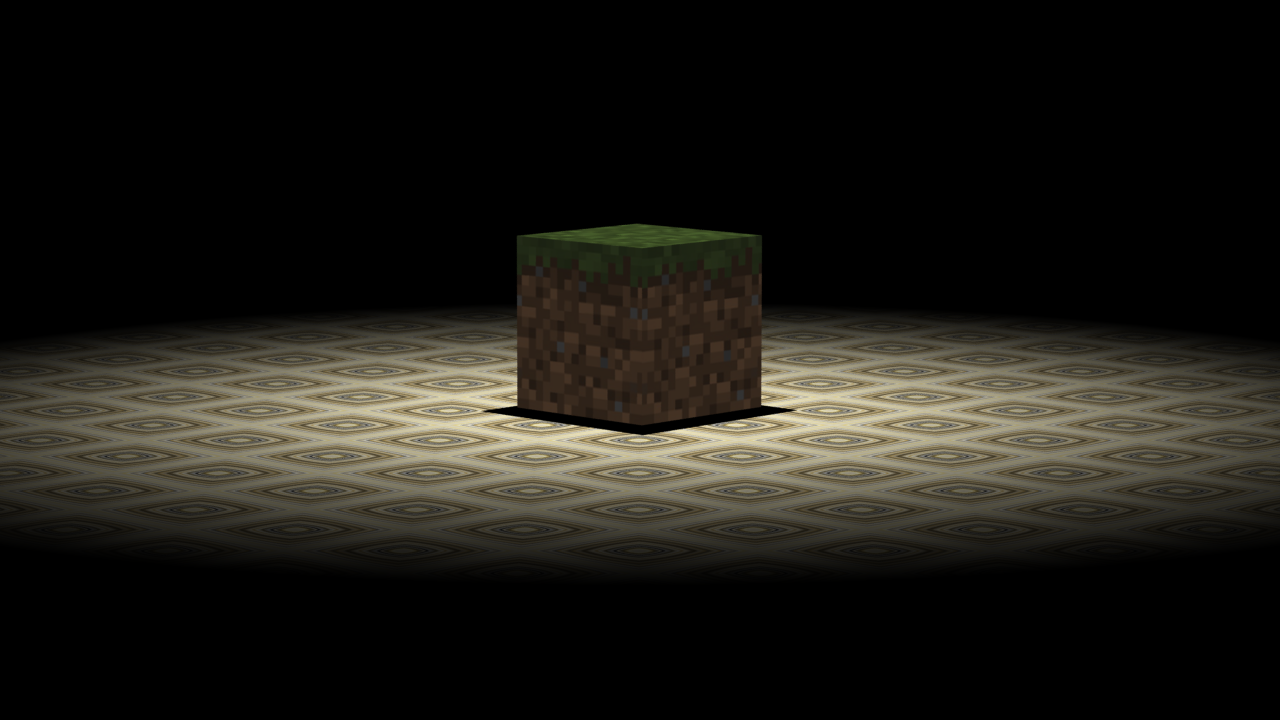
\includegraphics[width=\textwidth]{figures/processingTriangles.png}
\caption{Ray Casting Accomplished with Processing. One cube with twelve triangles and an image mapped to it on a plane with a repeated image texture illuminated by a spotlight.}
\label{fig:processingtriangles}
\end{figure}

\subsection{Performance Results}
For each test in Basic Ray Casting a variety of levels of complexity were tested in order to see how each language handles a different amount of load.  For each rendering a 1280 x 720 image size was used to generate a high quality image for testing.  The results are graphed and labeled in Figures \ref{fig:basicgraph} - \ref{fig:texgraph}.
\begin{figure}[ht]
\centering
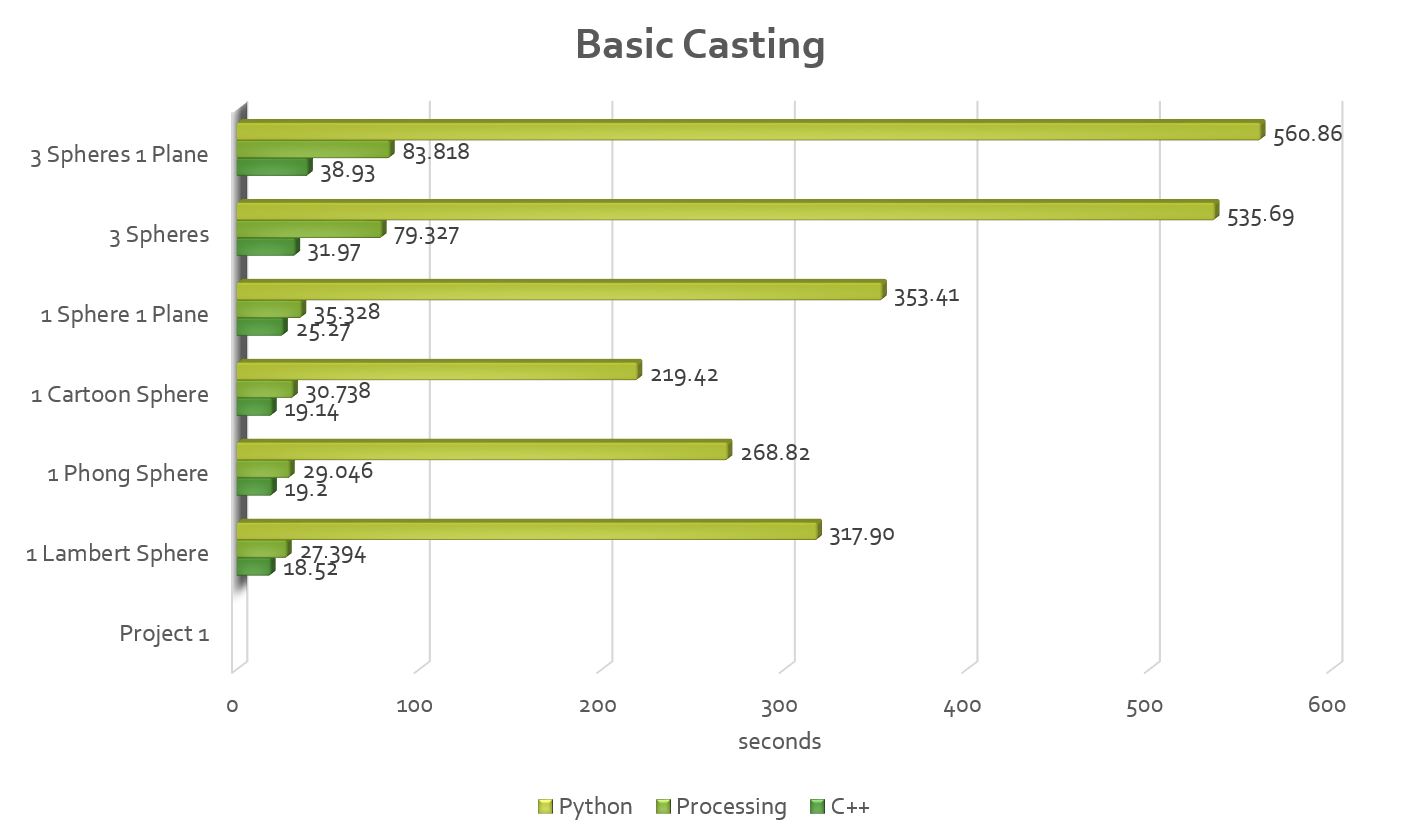
\includegraphics[width=\textwidth]{figures/graphs/basic-graph.png}
\caption{Basic ray tracing performance graph for each language}
\label{fig:basicgraph}
\end{figure}

\begin{figure}[ht]
\centering
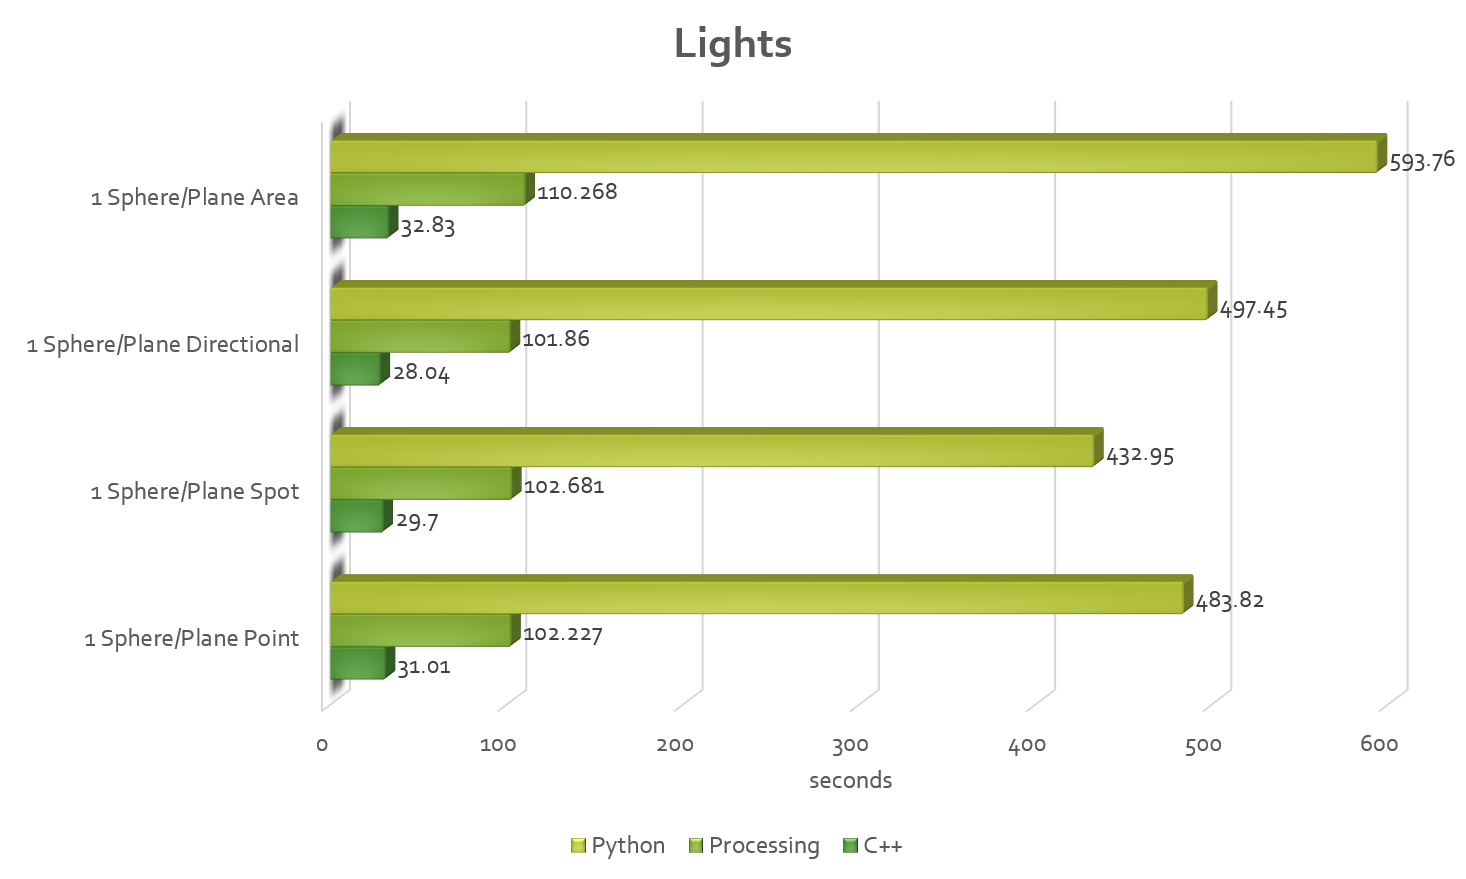
\includegraphics[width=\textwidth]{figures/graphs/lights-graph.png}
\caption{Light's performance graph for each language}
\label{fig:lightsgraph}
\end{figure}

\begin{figure}[ht]
\centering
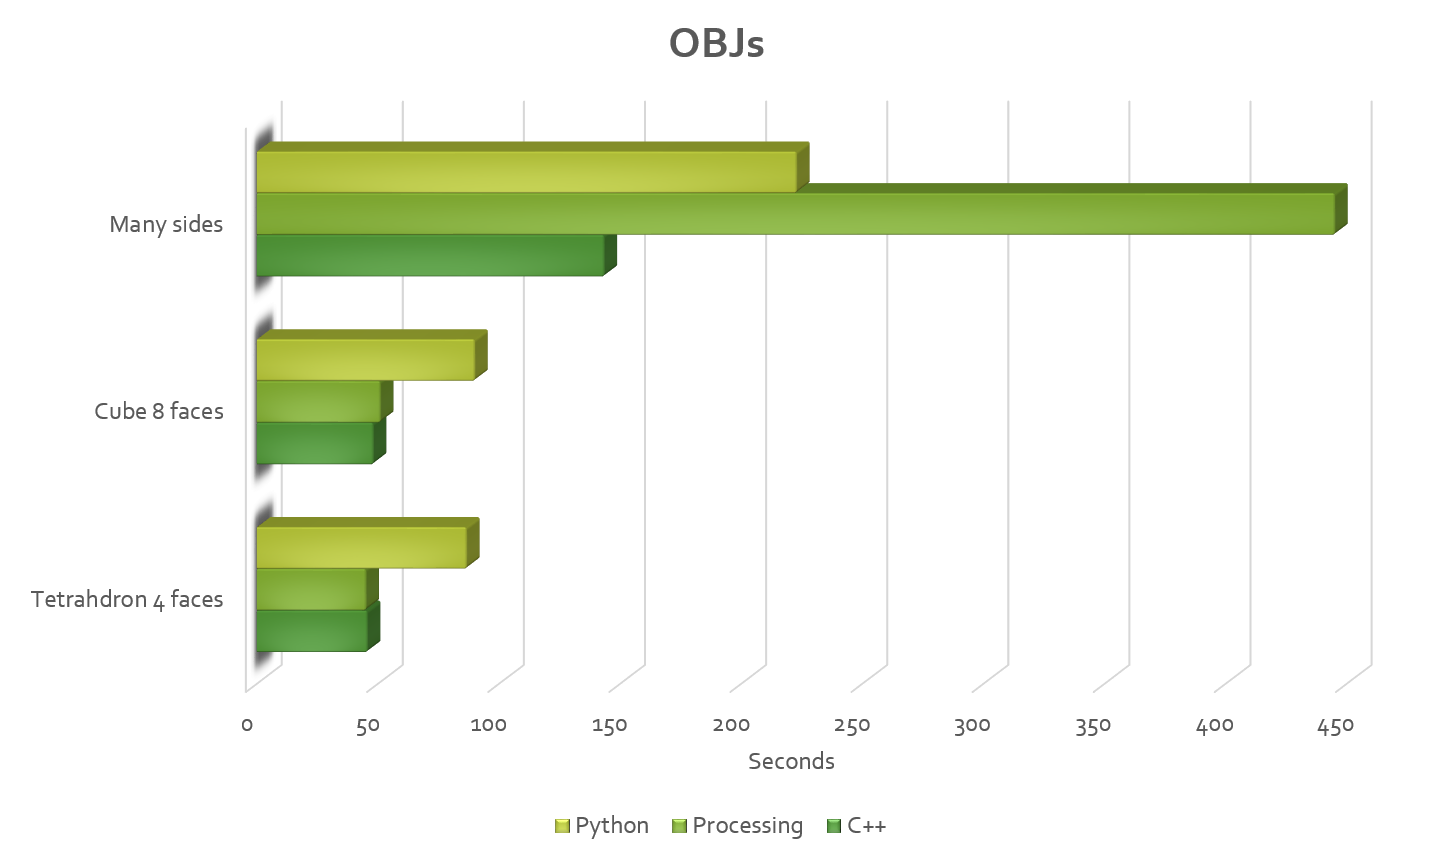
\includegraphics[width=\textwidth]{figures/graphs/obj-graph.png}
\caption{OBJ Performance Graph for each language}
\label{fig:objgraph}
\end{figure}

\begin{figure}[ht]
\centering
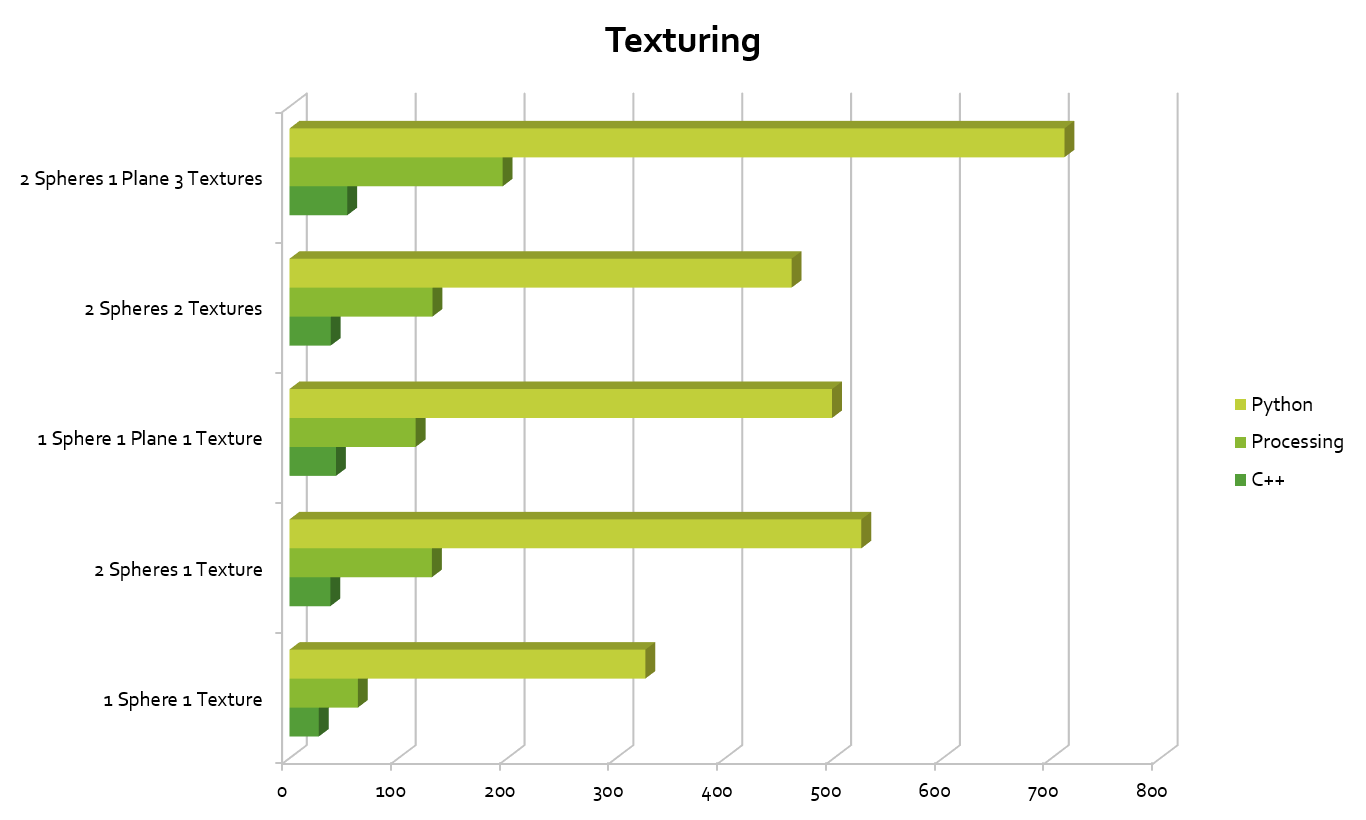
\includegraphics[width=\textwidth]{figures/graphs/texturing.png}
\caption{Texturing Performance Graph for each language}
\label{fig:texgraph}
\end{figure}

%%%%%%%%%%%%%%%%%%%%%%%%%%%%%%%%%%%%%%%%%%%%%%%%%%%%%%
%%%%%%%%%%%%%%%%%%%%%%%%%%%%%%%%%%%%%%%%%%%%%%%%%%%%%%
\section{Milestone 3: Ray Tracing and Distributed Ray Tracing}
The main complications discovered for this milestone where all related to the implementation of a recursive ray tracing strategy.  All three languages had the same difficulties that were not unique to each implementation.  To implement recursion requires the knowledge of establishing a process function within each raytracing function that will repeatedly call itself unless specific escape conditions are met.  It is important to establish these conditions such that they are met within the execution of the program or else the ray tracer will implement an infinite loop that will consume computing resources until the computer crashes and needs to be restarted.

The main challenge introduced for distributed ray tracing was the idea of randomness.  In order to get a jitter for every vector value for some aspect of the ray tracing process, whether it be the hit point or the view point of the camera.  To achieve this effect was different in each language, but Processing and Python were surprisingly similar.

\singlespacing
\begin{lstlisting}[language=C++, caption=C++ Random Function, style=mystyle, label=c++Rand]
float randNum(float LO, float HI)
{
    float U2 = LO + (float)rand()/((float)RAND_MAX/(HI-LO));
    return U2;
}
\end{lstlisting}
\begin{lstlisting}[language=Java, caption=Processing Random Function, style=mystyle, label=processingRand]
random(0.0,1.0);
\end{lstlisting}
\begin{lstlisting}[language=Python, caption=Python Random Function, style=mystyle, label=pythonRand]
random.uniform(0.0,1.0);
\end{lstlisting}
\doublespacing

Processing and Python each had their own random libraries that handled generating random numbers between two specified values but in C++ it was not provided.  Writing a random function took a lot of overhead and wasted time comprehending how computers generate random numbers in C++ at a foundational level.  It was significantly easier and more intuitive to implement a random function in both Python and Processing than it was in C++.

\subsection{Ray Tracing and Distributed Ray Tracing Images}
Here are a few images from the Ray Tracing and Distributed Ray Tracing Milestone.  While these are just a few examples from each language and each task, each language accomplished the same types of images that are presented in Figures \ref{fig:pyFlect} through \ref{fig:pyDist}.

\begin{figure}[ht]
\centering
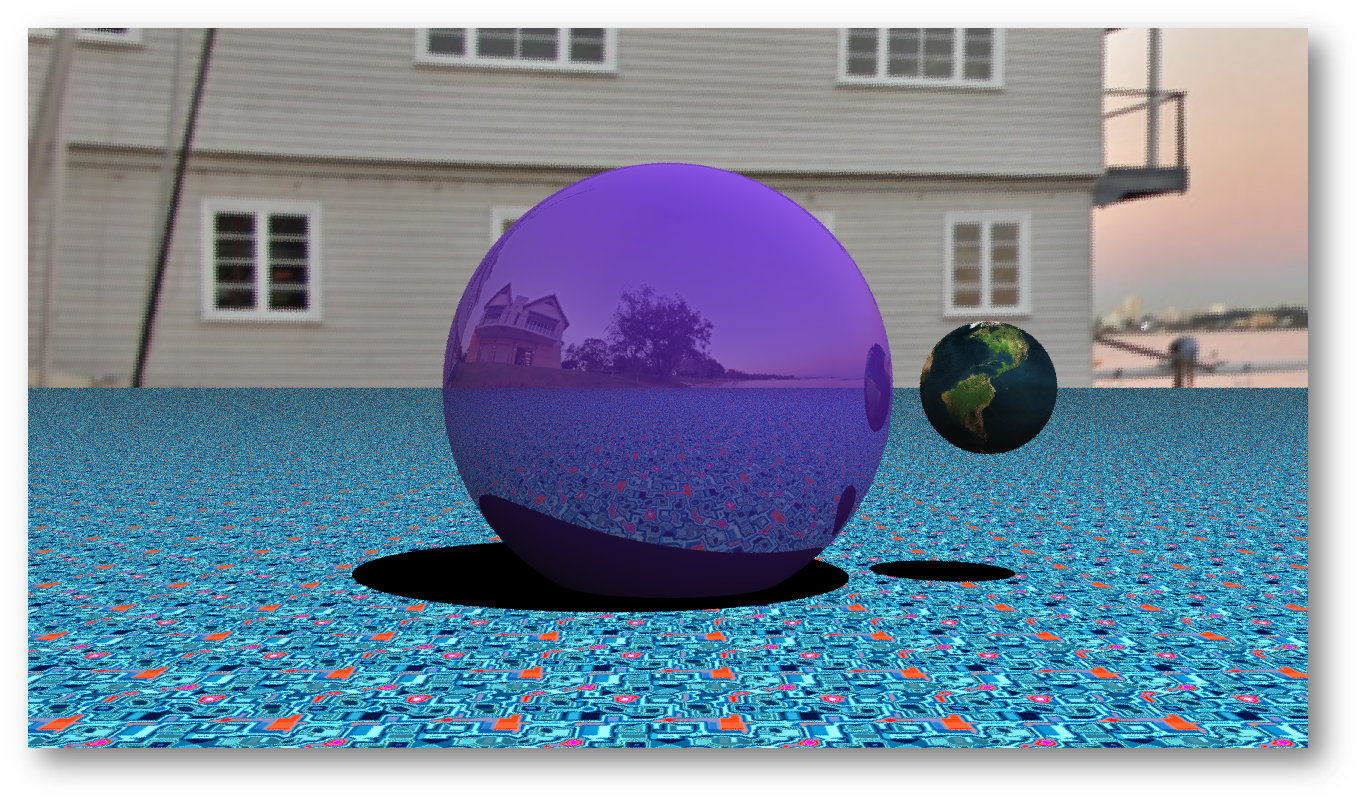
\includegraphics[width=\textwidth]{figures/python-reflection.png}
\caption{Reflection effect completed in Python}
\label{fig:pyFlect}
\end{figure}
\begin{figure}[ht]
\centering
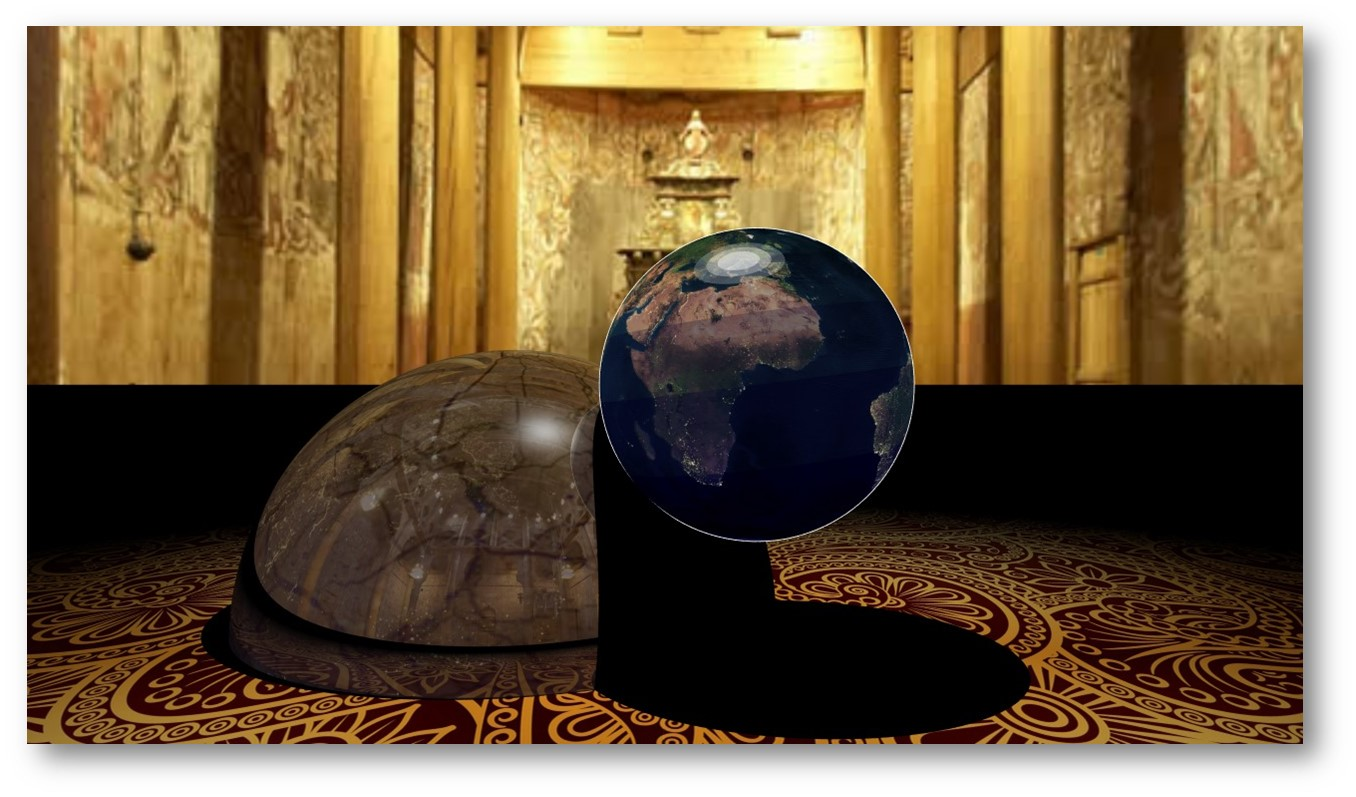
\includegraphics[width=\textwidth]{figures/c++-reflective.jpg}
\caption{Reflection Effect completed with C++}
\label{fig:c++Flect}
\end{figure}
\begin{figure}[ht]
\centering
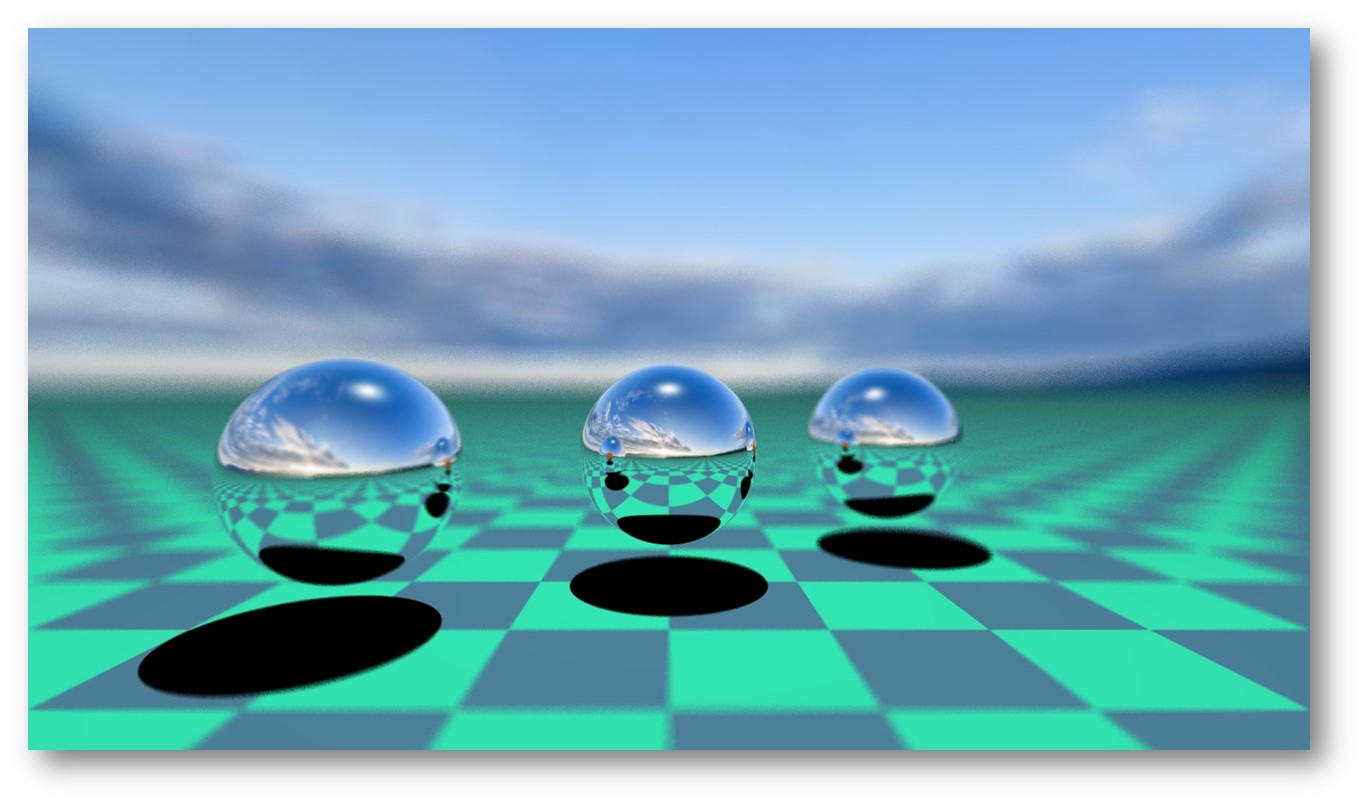
\includegraphics[width=\textwidth]{figures/c++-distributed.jpg}
\caption{Depth of Field effect captured with C++}
\label{fig:c++Dist}
\end{figure}
\begin{figure}[ht]
\centering
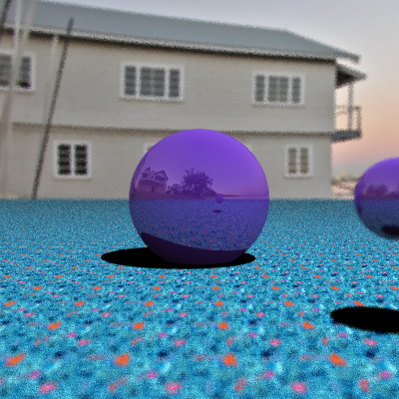
\includegraphics[width=300px]{figures/python-distributed.png}
\caption{Depth of Field effect captured with Python.  Pixelated image shows one of the restrictions of Python computing power for an image of this scale.}
\label{fig:pyDist}
\end{figure}

\subsection{Performance Results}
Performance results each language can be seen in Figure \ref{refGraph}
\begin{figure}[ht]
\centering
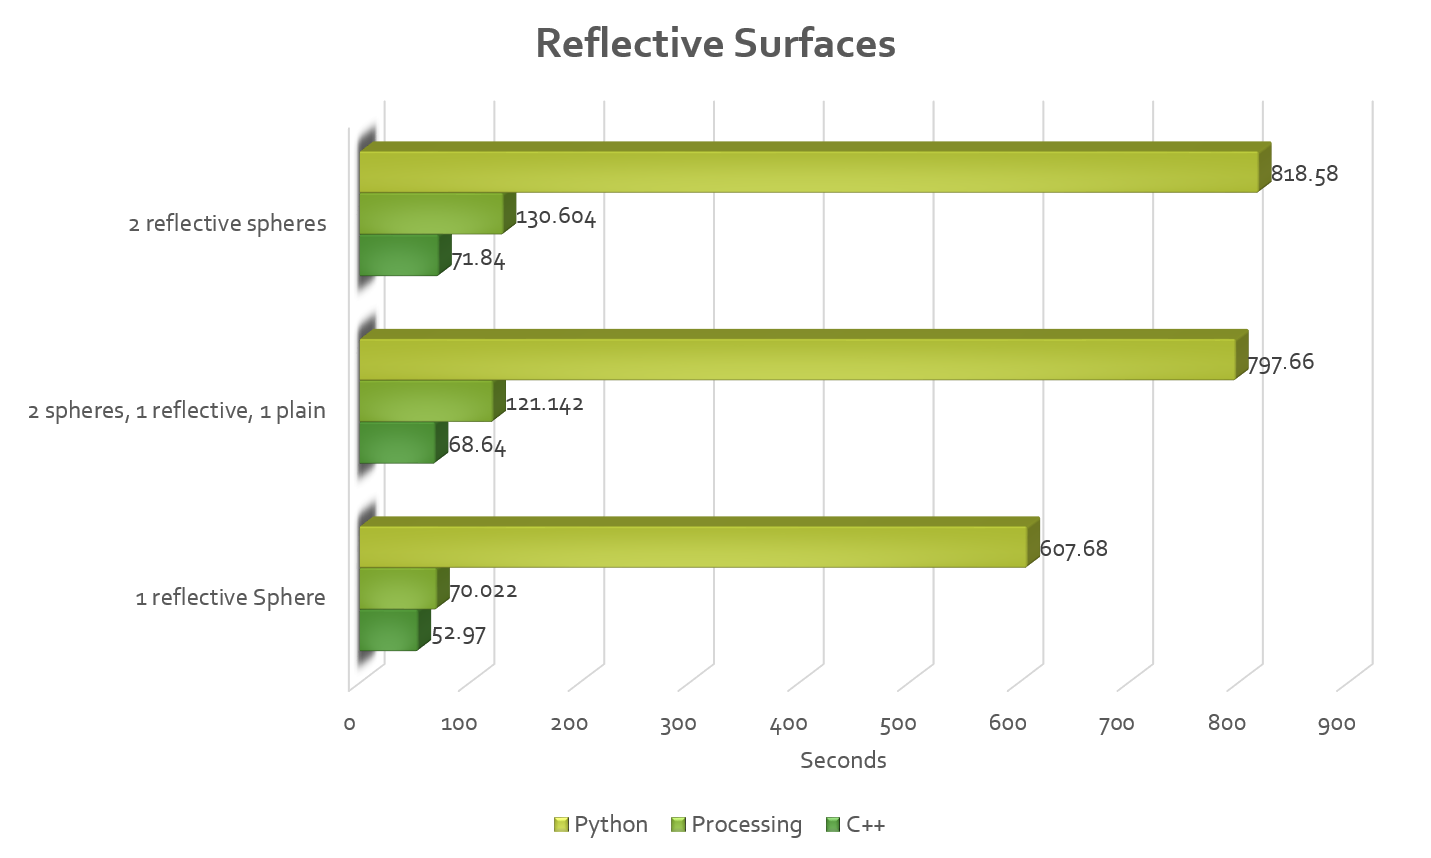
\includegraphics[width=\textwidth]{figures/graphs/reflective-graph.png}
\caption{Texturing Performance Graph for each language}
\label{fig:refGraph}
\end{figure}

\section{Milestone 4: Indirect Illumination}
Milestone 4 experienced the same complications as Milestone 3, with the majority of the implementation being the same throughout all three languages.  No new computer science concepts were introduced for this section, so this Milestone was completely based upon ray tracing theory rather than language implementation.  By this time I had fully mastered the languages and felt comfortable accomplishing the tasks in each.
\subsection{Indirect Illumination Images}
Images for the Indirect Illumintaion Milestone can be found in Figure \ref{fig:c++AO}.
\begin{figure}[ht]
\centering
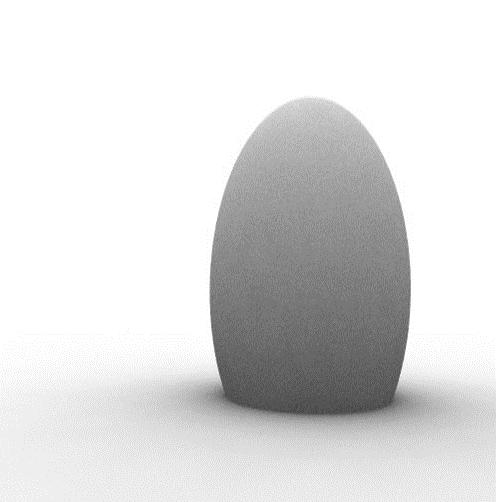
\includegraphics[width=\textwidth]{figures/indirectIllumination-c++.png}
\caption{Ambient Occlusion effect created with C++}
\label{fig:c++AO}
\end{figure}
